The training part provides 4 functionalities;

\begin{itemize}
\item \mintinline{python}{romc.solve_problems(n1, seed=None, use_bo=False)}
\item \mintinline{python}{romc.estimate_regions(epsilon)}
\item \mintinline{python}{romc.theta_hist(**kwargs)}
\item \mintinline{python}{romc.fit_posterior(n1, eps, quantile=None, use_bo=False, seed=None)}
\end{itemize}


\subsubsection*{API call (i): \pinline{romc.solve_problems(n1, seed=None, use_bo=False)}}

\noindent
The functionality is responsible for (a) drawing the nuisance
variables, (b) define the optimisation problems and (c) solve them
using either a gradient-based optimiser or Bayesian optimisation. The
aforementioned tasks are done in a sequential fashion, as show in
figure \ref{fig:elfi-model}. Passing an integer number as seed, makes
the random generation of the initial points deterministic, making the
whole process reproducible.

\subsubsection*{API call (ii): \pinline{romc.theta_hist(**kwargs)}}

This functionality can serve as an intermediate step of manual
inspection for choosing the threshold $\epsilon$. It plots a histogram
of the distances at the optimal point
$g_i(\thetab_i^* : \{i = 1, 2, ..., n_1\}$ hepling deciding a sensible
threshold. The function accepts all keyword arguments and forwards
them to the underlying \pinline{matplotlib.hist()} function; in this
way the user may customize some properties of the histogram, such as
the number of bins or the range of values.


\subsubsection*{API call (iii): \pinline{romc.estimate_regions(epsilon)}}

This functionality constructs the bounding boxes around the optimal
points $\thetab_i^* : \{ i = 1, 2, ..., n_1 \}$ following the
Algorithm \ref{alg:region_construction}. The hessian matrix is
approximated based on the jacobian $\hess_i = \jac_i^T \jac_i$ and the
eigenvectores are computed using the function
\pinline{numpy.linalg.eig()} that use the \pinline{_geev LAPACK} under
the hood. A check is performed so that the matrix $\hess_i$ is not
singular; if this is the case the orthonormal basis is returned as
eigenvectors. Afterwards, the limits are obtained by repeteadly
querying the distance function ($g_i(\thetab)$ or $\hat{d}(\thetab)$
depending on the optimisation scheme).


\subsubsection*{API call (iv): \pinline{romc.fit_posterior(n1, eps, quantile=None, use_bo=False, seed=None)}}

This functionality merges the three above into a single step. If the user doesn't want to manually inspect the histogram of the distances before deciding where to set the threshold $\epsilon$, he may call \pinline{romc.fit_posterior()} and the whole training process will be done end-to-end. There are two alternatives for setting the threshold $\epsilon$; the first is to set to a specific value blindly and the second is to set at as a specific quantile of the histogram of distances. In the second scenario the \pinline{quantile} argument must be set to a floating number in the range $[0,1]$ and \pinline{eps='auto'}.

\subsubsection*{\pinline{romc.visualize_region(i)}}
  
It can be used as an inspection utility for cases where the parametric space is $1D$ or $2D$, so that the visualization is feasible. The argument $\pinline{i}$ is the index of the corresponding optimization problem i.e.\ $i<n_1$.

\subsubsection*{Example}

Here we will illustrate the aforementioned functionalities using the simple 1D example we set up in the previous chapter. The code snippet that implements those steps using a gradient-based approach, is the following;

\begin{minted}
[framesep=2mm,
baselinestretch=1.2,
fontsize=\small,
]
{python}
  '''Training part snippet'''
  n1 = 100
  seed = 21
  eps = .75
  use_bo = False # True, if using Bayesian optimisation

  # Training set-by-step
  romc.solve_problems(n1=n1, seed=seed, use_bo=use_bo)
  romc.theta_hist(bins=100)
  romc.estimate_regions(eps=eps)
  romc.visualize_region(i=1)

  # Equivalent one-line command
  # romc.fit_posterior(n1=n1, eps=eps, use_bo=use_bo, seed=seed)
\end{minted}


We observe that all optimal points produce zero distance, thus the histogram has mass only at zero. For observing the curve around the optimal point and the acceptance region of the first optimisation problem. We observe the switching to the alternative Bayesian optimisation scheme needs nothing more the setting the argument \pinline{use_bo=True}; all the following command remain unchanged. If the practitioner doesn't want to observe the histogram of the distances for setting the threshold $\epsilon$, the command \pinline{romc.fit_posterior()} is a single-line equivalent.

\begin{figure}[h]
    \begin{center}
      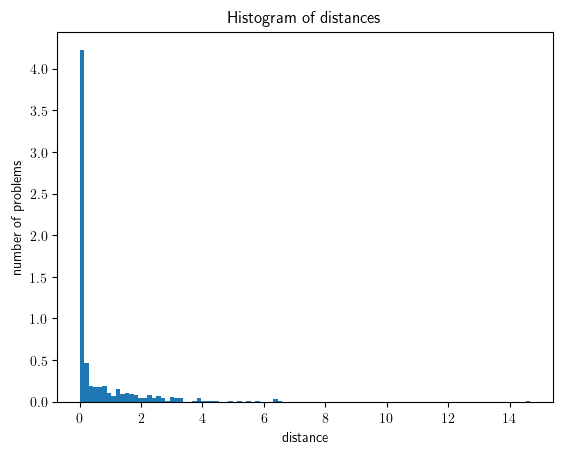
\includegraphics[width=0.48\textwidth]{./Thesis/images/chapter3/example_theta_dist.png}
      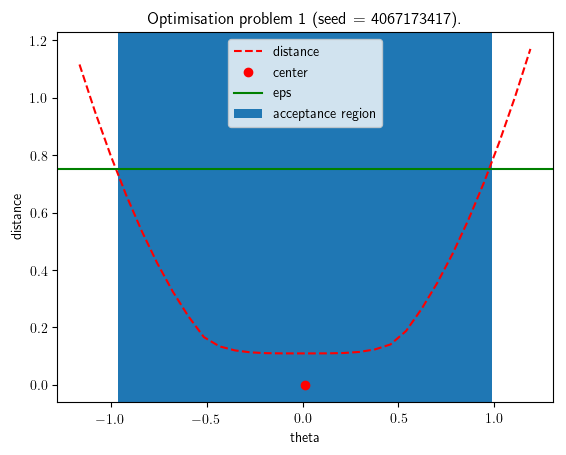
\includegraphics[width=0.48\textwidth]{./Thesis/images/chapter3/example_region.png}
    \end{center}
  \caption{Histogram of distances and visualisation of a specific region.}
  \label{fig:example_training}
\end{figure}
